%!TEX root = ./template-skripsi.tex
%-------------------------------------------------------------------------------
%                            BAB II
%                          KAJIAN TEORI
%-------------------------------------------------------------------------------

\chapter{KAJIAN PUSTAKA}

\section{Pengertian Citra Digital}
  Citra digital adalah representasi visual dari objek atau pemandangan yang diwakili dalam bentuk data numerik.
Sebuah citra dapat didefinisikan sebagai fungsi dua dimensi, \(f(x, y)\), di mana \(x\) dan \(y\) adalah koordinat spasial (bidang), dan amplitudo \(f\) pada setiap pasangan koordinat \((x, y)\) disebut intensitas atau tingkat keabuan citra pada titik tersebut. Ketika \(x\), \(y\), dan nilai intensitas \(f\) semuanya merupakan besaran yang terbatas dan diskret, maka citra tersebut disebut citra digital. Bidang pengolahan citra digital mengacu pada pemrosesan citra digital dengan menggunakan komputer digital (\cite[hlm. 1--6]{Gonzalez2018}).

\section{Pengolahan Citra Digital}
  Pengolahan citra digital adalah proses manipulasi citra digital untuk meningkatkan kualitas, mengubah representasi, atau mengekstrak informasi yang berguna. Proses ini melibatkan berbagai teknik dan algoritma yang dapat digunakan untuk mengolah citra, seperti penghalusan, peningkatan kontras, deteksi tepi, dan segmentasi. Pengolahan citra digital memiliki aplikasi luas dalam berbagai bidang, termasuk pengenalan pola, visi komputer, dan analisis citra medis (\cite[hlm. 27--32]{Gonzalez2018}). 
  Salah satu tahapan penting dalam pengolahan citra adalah konversi citra ke dalam bentuk grayscale sebelum dilakukan ekstraksi fitur atau deteksi tepi (\cite[hlm. 307--308]{Sanchez2018}).

\section{Citra Grayscale}
  Citra grayscale adalah representasi citra yang hanya menggunakan satu saluran warna, yaitu tingkat keabuan. Citra ini dihasilkan dengan mengubah citra berwarna menjadi skala abu-abu, di mana setiap piksel dalam citra hanya memiliki nilai intensitas yang mewakili tingkat keabuan. Proses ini sering dilakukan untuk menyederhanakan analisis citra, karena mengurangi kompleksitas data yang harus diproses (\cite[hlm. 27--32]{Gonzalez2018}). 
  Penggunaan citra grayscale sangat umum dalam proses deteksi fitur multi-skala dan algoritma deteksi sudut seperti Harris-Corner Detection, karena memudahkan perhitungan gradien dan matriks momen kedua (\cite[hlm. 307--308]{Sanchez2018}).

\section{Multi-Scale Feature Detection}
  Deteksi fitur multi-skala adalah pendekatan yang digunakan untuk mendeteksi fitur pada berbagai skala dalam citra. Pendekatan ini penting karena objek dalam citra dapat muncul pada berbagai ukuran, dan deteksi fitur yang efektif harus mampu mengenali objek tersebut terlepas dari skala yang digunakan. Salah satu metode yang umum digunakan dalam deteksi fitur multi-skala adalah \emph{Gaussian Pyramid}, di mana citra asli dihaluskan dan diperkecil untuk membuat serangkaian citra dengan resolusi yang berbeda. Dengan cara ini, fitur dapat diekstraksi dari setiap tingkat piramida, memungkinkan deteksi yang lebih robust terhadap perubahan skala (\cite[hlm. 91--92]{Lowe2004}).

\subsection{Gaussian scale-space}

Dalam domain diskrit citra digital, parameter skala juga direpresentasikan secara diskrit. 
Dengan demikian, representasi ruang-skala merupakan kumpulan gambar yang direpresentasikan oleh perbedaan tingkat resolusi diskrit. 
Sebuah penelitian menunjukkan bahwa ruang-skala harus memenuhi persamaan yang dapat dicapai melalui konvolusi dengan kernel Gaussian. 
Selanjutnya, penelitian tersebut memperlihatkan bahwa kernel Gaussian adalah satu-satunya kernel unik yang dapat menghasilkan representasi skala-ruang. 
Keunikan kernel Gaussian ini telah dikonfirmasi melalui berbagai formulasi dalam sejumlah penelitian lain (\cite[hlm. 92--93]{Lowe2004}; \cite[hlm. 13--15]{mikolajczyk:tel-00584096}). 
Temuan ini menyimpulkan bahwa konvolusi dengan kernel Gaussian merupakan solusi optimal untuk masalah konstruksi representasi multi-skala. Fungsi Gaussian dua dimensi didefinisikan sebagai berikut:

\begin{equation*}
g(\sigma) = \frac{1}{2\pi\sigma_{x}\sigma_{y}}\exp\left(-\frac{(x^2+\mu_{x})+(y^2+\mu_{y})}{2\sigma_{x}\sigma_{y}}\right)
\end{equation*}

Jika \(\mu_{x} = \mu_{y} = 0\) dan \(\sigma_{x} = \sigma_{y}\) maka dapat disederhanakan menjadi :
\begin{equation}
g(\sigma) = \frac{1}{2\pi\sigma^2}\exp\left(-\frac{x^2+y^2}{2\sigma^2}\right)
\label{eq:gaussian kernel}
\end{equation}

Keunikan dari kernel Gaussian dapat diketahui dari beberapa sifat berikut : 
\emph{linearity, separability, causality, and semi group property.} Keterpisahan 
atau \emph{separability} memungkinan \emph{multi-dimensional Gaussian kernel} diperoleh sebagai hasil perkalian kernel satu dimensi:

\begin{equation*}
  g(x,y) = g(x)g(y)
\end{equation*}

Sifat ini sangat berguna dalam praktik karena penghalusan sinyal dua dimensi dapat digantikan oleh dua penghalusan satu dimensi, satu untuk setiap dimensi (\cite[hlm. 92]{Lowe2004}). 
Filter Gaussian satu dimensi dapat diimplementasikan sebagai filter rekursif, yang secara signifikan mempercepat proses 
komputasi pada kasus kernel Gaussian yang lebih besar (yaitu > \( \sqrt{2}\)). 
Kondisi kausalitas menyatakan bahwa tidak ada struktur tambahan atau buatan yang dibuat saat menghitung citra pada skala kasar, 
yaitu citra pada skala yang lebih kasar merupakan representasi yang disederhanakan dari citra pada skala yang lebih halus (\cite[hlm. 13--14]{mikolajczyk:tel-00584096}). 
Sifat semi-grup komutatif menyatakan bahwa \(n\) kali penghalusan berturut-turut pada sebuah citra akan memberikan hasil yang sama dengan satu kali penghalusan menggunakan ukuran kernel yang sama dengan jumlah seluruh \(n\) kernel tersebut. 
Selain itu, operasi \(n\) tersebut dapat dilakukan dalam urutan apa pun:

\begin{equation*}
g(\sigma_{1}) * \cdots * g(\sigma_{n}) * I(x) = g(\sigma_{1} + \cdots + \sigma_{n}) * I(x)
\end{equation*}

Biasanya, ruang-skala yang seragam digunakan, tetapi representasi ruang-skala yang lebih umum dihitung menggunakan filter afine (\cite[hlm. 14--15]{mikolajczyk:tel-00584096}).

\textbf{Uniform scale-space}. Perbedaan tingkat pada representasi ruang-skala secara umum, terbuat dari konvolusi dengan \emph{gaussian kernel} :

\begin{equation}
L(x,\sigma) = g(\sigma) * I(x)
\label{eq:konvolusi}
\end{equation}

Dengan \(I\) adalah gambar dan \(x = (x,y)\) adalah lokasi poin.
\emph{Kernel} adalah simetris sirkular dan diparameterisasi dari satu skala faktor \(\sigma \).

\begin{figure}
  \centering{}
  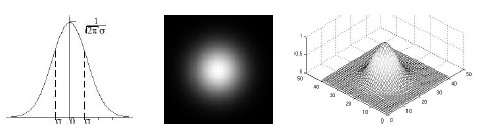
\includegraphics[width=0.8\textwidth]{gambar/Uniform Gaussian kernel.jpg}
  \caption{}
\end{figure}

\section{\emph{Gradient}}
  Gradien dalam matematika dan pemrosesan citra adalah sebuah konsep yang menunjukkan arah perubahan sebuah nilai intensitas pada suatu titik pada gambar 2-Dimensi atau 3-Dimensi. 
Dalam gambar atau citra digital, Gradien memainkan peran utama dalam membentuk matriks auto-korelasi, yang nilai eigennya menggambarkan struktur lokal gambar. 
Wilayah dengan nilai eigen tinggi di semua arah menunjukkan sudut, sedangkan wilayah dengan satu nilai eigen tinggi menggambarkan tepi (\cite[hlm. 305--306]{Sanchez2018}).

  Berbagai operator gradien, seperti Sobel, Prewitt, dan Scharr, digunakan untuk menghitung gradien dalam gambar dengan mendeteksi perubahan intensitas piksel di sepanjang arah tertentu. 
Operator Sobel, sebagai salah satu metode yang paling umum, menggunakan kernel konvolusi untuk menghitung gradien dalam arah horizontal (x) dan vertikal (y), menghasilkan peta gradien yang mengidentifikasi tepi dan perubahan penting dalam struktur gambar.
\subsection{Operator Sobel}
  Operator Sobel adalah salah satu metode yang paling umum digunakan untuk menghitung gradien dalam citra digital. Metode ini menggunakan dua kernel konvolusi, satu untuk mendeteksi perubahan horizontal dan satu lagi untuk perubahan vertikal. Kernel ini dirancang untuk memberikan bobot lebih pada piksel yang berada di tengah, sehingga lebih sensitif terhadap perubahan intensitas yang tajam.
\begin{equation}
  S_x = \begin{bmatrix}
    -1 & 0 & 1 \\
    -2 & 0 & 2 \\
    -1 & 0 & 1
  \end{bmatrix}, \quad
  S_y = \begin{bmatrix}
    1 & 2 & 1 \\
    0 & 0 & 0 \\
    -1 & -2 & -1
  \end{bmatrix}
\end{equation}

  Dengan menggunakan kernel ini, gradien dalam arah x dan y dapat dihitung dengan mengkonvolusi citra dengan masing-masing kernel. Hasilnya adalah dua peta gradien yang menunjukkan perubahan intensitas dalam arah horizontal dan vertikal. Magnitudo gradien dapat dihitung dengan rumus berikut:

\begin{equation}
  G = \sqrt{G_x^2 + G_y^2}
\end{equation}

  Di mana \(G_x\) dan \(G_y\) adalah hasil konvolusi citra dengan kernel Sobel untuk arah x dan y. Peta gradien ini sangat berguna dalam deteksi tepi, segmentasi citra, dan ekstraksi fitur, karena membantu mengidentifikasi area dengan perubahan intensitas yang signifikan (\cite[hlm. 306--307]{Sanchez2018}).

\section{\emph{Second moment matrix}}
  Matriks momen kedua (\emph{second moment matrix}) adalah matriks simetris 2x2 yang mencerminkan variasi intensitas di sekitar piksel dalam sebuah citra. Matriks ini seringkali digunakan untuk mendeteksi fitur, atau mendeskripsikan struktur dari \emph{local image}.
Matriks ini juga panggil sebagai matriks auto-korelasi, seperti pada rumus \ref{eq:SecondMomentMatrix}

\begin{equation}
  M = 
    \begin{bmatrix}
      A & C \\
      C & B
    \end{bmatrix}
    = g(\sigma_{I}) *
      \begin{bmatrix}
        I_{x}^2 & I_{x}I_{y} \\
        I_{x}I_{y} & I_{y}^2
      \end{bmatrix}
  \label{eq:SecondMomentMatrix}
\end{equation}

Hasil dari turunan dihitung pada setiap posisi dan koefisien dari matriks dikonvolusi dengan fungsi gaussian. Langkah ini merupakan langkah paling lama karena menggunakan tiga konvolusi Gaussian (\cite[hlm. 307]{Sanchez2018}). 

Matriks ini memiliki dua nilai eigen, yang memungkinkan identifikasi suatu area sebagai berikut:

\begin{itemize}
  \item Jika kedua nilai eigen kecil, maka area tersebut adalah \emph{flat area}.
  \item Jika satu nilai besar, dan satu kecil, maka area tersebut adalah tepi.
  \item Jika kedua nilai eigen besar, maka kemungkinan besar area tersebut adalah sudut (\emph{corner}).
\end{itemize}

Dengan menggunakan sifat tersebut, respon sudut dapat dihitung menggunakan analisis nilai eigen atau metode lain, salah satunya fungsi kekuatan sudut Harris \(R\) seperti yang dijelaskan pada rumus \ref{Harris-Corner Detection}.

\section{\emph{Harris-Corner Detection}}
  \emph{Harris-Corner Detection} merupakan salah satu dari sekian banyak algoritma untuk mendeteksi fitur (\emph{feature}), algoritma ini pertama kali diperkenalkan oleh Chris Harris dan Mike Stephens pada tahun 1988 (\cite{Harris2013}). 
Ide dibalik metode Harris adalah untuk mendeteksi titik sudut berdasarkan variasi intensitas di area sekitar: wilayah yang kecil di sekitar fitur menunjukkan perubahan intensitas yang besar dibandingkan dengan pergeseran jendela ke segala arah (\cite[hlm. 305--308]{Sanchez2018}).
Dengan melibatkan matriks momen kedua (\emph{second moment matrix}) untuk menghitung variasi perubahan intensitas dalam dua arah utama.

\begin{equation}
  R = det(M) - k * (trace(M))^2
  \label{Harris-Corner Detection}
\end{equation}

  Nilai \(R\) akan menunjukkan keberadaan sudut pada area tersebut. 
Jika nilai \(R\) yang besar akan menunjukkan keberadaan sudut di area tersebut, sebaliknya nilai \(R\) yang kecil menunjukkan daerah tersebut merupakan tepi.

\section{Euclidean dan Interpolasi}
  Pada pengolahan citra digital, perhitungan jarak atau panjang antara dua titik sangat penting untuk berbagai aplikasi, seperti pengukuran objek, deteksi fitur, dan transformasi citra. Dua metode dasar yang sering digunakan adalah rumus Euclidean dan interpolasi.

  \textbf{Euclidean} merupakan cara paling dasar untuk mengukur jarak lurus antara dua titik dalam ruang dua dimensi. Rumus ini didasarkan pada teorema Pythagoras, di mana jarak antara dua titik \(P_1(x_1, y_1)\) dan \(P_2(x_2, y_2)\) dihitung sebagai:
\begin{equation}
  d = \sqrt{(x_2 - x_1)^2 + (y_2 - y_1)^2}
  \label{eq:euclidean}
\end{equation}
  Dengan \(d\) adalah jarak Euclidean antara dua titik. Rumus ini juga dapat diperluas ke dimensi yang lebih tinggi dan digunakan secara luas untuk mengukur kedekatan atau kemiripan antara dua piksel atau fitur pada citra (\cite[hlm. 34]{Gonzalez2018}).

  \textbf{Interpolasi} adalah metode untuk memperkirakan nilai di antara dua atau lebih titik data yang diketahui. Dalam konteks citra digital, interpolasi digunakan untuk menentukan nilai intensitas piksel pada posisi yang tidak tepat berada pada grid piksel, misalnya saat melakukan rotasi, penskalaan, atau transformasi citra. Selain itu, interpolasi juga dapat digunakan untuk menghitung nilai berat (weight) pada titik-titik tertentu, seperti dalam operasi filter atau penyesuaian nilai piksel hasil transformasi. Salah satu contoh rumus interpolasi linier untuk dua titik adalah:
\begin{equation}
  f(x) = f(x_0) + \frac{(x - x_0)}{(x_1 - x_0)} \left[ f(x_1) - f(x_0) \right]
  \label{eq:interpolasi-linier}
\end{equation}
  Untuk interpolasi bilinear pada citra dua dimensi, nilai pada titik \((x, y)\) di antara empat piksel tetangga dapat dihitung dengan:
\begin{equation*}
  f(x, y) = a_0 + a_1x + a_2y + a_3xy
  \label{eq:interpolasi-bilinear}
\end{equation*}
  di mana koefisien \(a_0, a_1, a_2, a_3\) ditentukan berdasarkan nilai intensitas keempat piksel tetangga. Metode interpolasi ini sangat penting dalam proses resampling, rotasi, transformasi citra, maupun dalam perhitungan bobot piksel pada berbagai algoritma pengolahan citra (\cite[hlm. 89--91]{Gonzalez2018}).





